\documentclass[border=6pt]{standalone}
\usepackage{tikz}
\usepackage[edges]{forest}
\usetikzlibrary{arrows.meta,positioning,calc,decorations.pathreplacing,shapes.geometric}
\begin{document}
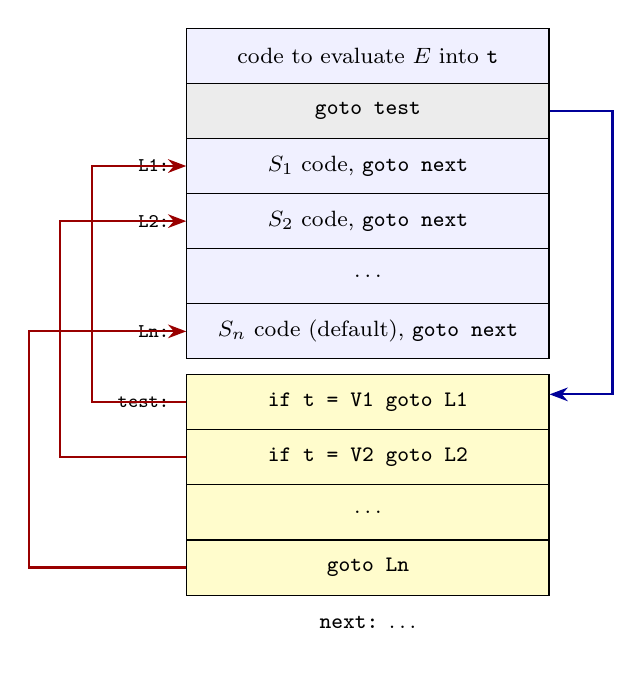
\begin{tikzpicture}[>=Stealth,font=\small,
 cell/.style={draw,minimum width=4.6cm,minimum height=0.7cm,align=center,font=\footnotesize},
 lab/.style={font=\scriptsize\ttfamily,anchor=east}]
\node[cell,fill=blue!6] (e) at (0,0) {code to evaluate $E$ into \texttt{t}};
\node[cell,fill=gray!15] (g) at (0,-0.7) {\texttt{goto test}};
\node[cell,fill=blue!6] (s1) at (0,-1.4) {$S_1$ code, \texttt{goto next}};
\node[cell,fill=blue!6] (s2) at (0,-2.1) {$S_2$ code, \texttt{goto next}};
\node[cell,fill=blue!6] (sd) at (0,-2.8) {$\ldots$};
\node[cell,fill=blue!6] (sn) at (0,-3.5) {$S_n$ code (default), \texttt{goto next}};
\node[cell,fill=yellow!20] (t1) at (0,-4.4) {\texttt{if t = V1 goto L1}};
\node[cell,fill=yellow!20] (t2) at (0,-5.1) {\texttt{if t = V2 goto L2}};
\node[cell,fill=yellow!20] (td) at (0,-5.8) {$\ldots$};
\node[cell,fill=yellow!20] (tg) at (0,-6.5) {\texttt{goto Ln}};
\node[cell,draw=none] (nx) at (0,-7.2) {\texttt{next:} $\ldots$};
\node[lab] at (-2.4,-1.4) {L1:}; \node[lab] at (-2.4,-2.1) {L2:}; \node[lab] at (-2.4,-3.5) {Ln:};
\node[lab] at (-2.4,-4.4) {test:};
\draw[->,thick,blue!60!black] (g.east) -- ++(0.8,0) |- ([yshift=0.1cm]t1.east);
\draw[->,thick,red!60!black] (t1.west) -- ++(-1.2,0) |- (s1.west);
\draw[->,thick,red!60!black] (t2.west) -- ++(-1.6,0) |- (s2.west);
\draw[->,thick,red!60!black] (tg.west) -- ++(-2.0,0) |- (sn.west);
\end{tikzpicture}
\end{document}
